%!TEX root=lab1.tex
% mainfile: lab1.tex
% CS 580 style
% Typical usage (all UPPERCASE items are optional):
%       \input 580pre
%       \begin{document}
%       \MYTITLE{Title of document, e.g., Lab 1\\Due ...}
%       \MYHEADERS{short title}{other running head, e.g., due date}
%       \PURPOSE{Description of purpose}
%       \SUMMARY{Very short overview of assignment}
%       \DETAILS{Detailed description}
%         \SUBHEAD{if needed} ...
%         \SUBHEAD{if needed} ...
%          ...
%       \HANDIN{What to hand in and how}
%       \begin{checklist}
%       \item ...
%       \end{checklist}
% There is no need to include a "\documentstyle."
% However, there should be an "\end{document}."
%
%===========================================================
\documentclass[11pt,twoside,titlepage]{article}
%%NEED TO ADD epsf!!
\usepackage{../assets/threeparttop}
\usepackage{graphicx}
\usepackage{latexsym}
\usepackage{color}
\usepackage{listings}
\usepackage{fancyvrb}
%\usepackage{pgf,pgfarrows,pgfnodes,pgfautomata,pgfheaps,pgfshade}
%\usepackage{tikz}
%\usepackage[normalem]{ulem}
%\tikzset{
%    %Define standard arrow tip
%    >=stealth',
%    %Define style for boxes
%    oval/.style={
%           rectangle,
%           rounded corners,
%           draw=black, very thick,
%           text width=6.5em,
%           minimum height=2em,
%           text centered},
%    % Define arrow style
%    arr/.style={
%           ->,
%           thick,
%           shorten <=2pt,
%           shorten >=2pt,}
%%%}
\usepackage[noend]{algorithmic}
\usepackage[noend]{algorithm}
\newcommand{\bfor}{{\bf for\ }}
\newcommand{\bthen}{{\bf then\ }}
\newcommand{\bwhile}{{\bf while\ }}
\newcommand{\btrue}{{\bf true\ }}
\newcommand{\bfalse}{{\bf false\ }}
\newcommand{\bto}{{\bf to\ }}
\newcommand{\bdo}{{\bf do\ }}
\newcommand{\bif}{{\bf if\ }}
\newcommand{\belse}{{\bf else\ }}
\newcommand{\band}{{\bf and\ }}
\newcommand{\breturn}{{\bf return\ }}
\newcommand{\mod}{{\rm mod}}
\renewcommand{\algorithmiccomment}[1]{$\rhd$ #1}
\newenvironment{checklist}{\par\noindent\hspace{-.25in}{\bf Checklist:}\renewcommand{\labelitemi}{$\Box$}%
\begin{itemize}}{\end{itemize}}
\pagestyle{threepartheadings}
\usepackage{url}
\usepackage{wrapfig}
% removing the standard hyperref to avoid the horrible boxes
%\usepackage{hyperref}
\usepackage[hidelinks]{hyperref}
% added in the dtklogos for the bibtex formatting
\usepackage{dtklogos}
%=========================
% One-inch margins everywhere
%=========================
\setlength{\topmargin}{0in}
\setlength{\textheight}{8.5in}
\setlength{\oddsidemargin}{0in}
\setlength{\evensidemargin}{0in}
\setlength{\textwidth}{6.5in}
%===============================
%===============================
% Macro for document title:
%===============================
\newcommand{\MYTITLE}[1]%
   {\begin{center}
     \begin{center}
     \bf
     CMPSC 250 \\ Analysis of Algorithms
     \medskip
     \end{center}
     \bf
     #1
     \end{center}
}
%================================
% Macro for headings:
%================================
\newcommand{\MYHEADERS}
   {
   \lhead{\today}
   \rhead{Willem Yarbrough \& Curtis Aldean}
    %\immediate\write16{}
    %\immediate\write16{DATE OF HANDOUT?}
    %\read16 to \dateofhandout
    %\immediate\write16{}
    %\immediate\write16{HANDOUT NUMBER?}
    %\read16 to\handoutnum
   }

%================================
% Macro for bold italic:
%================================
\newcommand{\bit}[1]{{\textit{\textbf{#1}}}}

%=========================
% Non-zero paragraph skips.
%=========================
\setlength{\parskip}{1ex}

%=========================
% Create various environments:
%=========================
\newcommand{\PURPOSE}{\par\noindent\hspace{-.25in}{\bf Purpose:\ }}
\newcommand{\SUMMARY}{\par\noindent\hspace{-.25in}{\bf Summary:\ }}
\newcommand{\DETAILS}{\par\noindent\hspace{-.25in}{\bf Details:\ }}
\newcommand{\HANDIN}{\par\noindent\hspace{-.25in}{\bf Hand in:\ }}
\newcommand{\SUBHEAD}[1]{\bigskip\par\noindent\hspace{-.1in}{\sc #1}\\}
%\newenvironment{CHECKLIST}{\begin{itemize}}{\end{itemize}}


\usepackage{amsmath}
\usepackage{setspace}
\usepackage{amssymb}
\usepackage{amsthm}
\usepackage{listings}
\usepackage{tikz}
\usepackage{csvsimple}
\usepackage{minted}
\usepackage{fancyvrb}
\usepackage{multicol}
%\usepackage{minipage}
% \usetikzlibrary{automata,positioning}
\setlength{\parindent}{0pt}

\lstset{breaklines=true, showstringspaces=false,
    basicstyle=\footnotesize\ttfamily
}

\begin{document}
\doublespacing

\MYHEADERS
\MYTITLE{Final Project Writeup}

    \section{Motivation}
      For our CMPSC 250 Final Project, we decided to implement the
      quadtree data structure and apply it to 2D collision detection to
      evaluate the performance gains offered by using spatial indexing
      to reduce computation over a brute-force algorithm. Collision
      detection is commonly used in simulation environments, to detect
      if two objects are colliding (and to subsequently apply some
      computation to the objects in question). As such, we chose to
      visualize the efficiency of our quadtree implementation by
      rendering a 2D environment of particles to the screen.  \par This
      project employs a similar scheme to the lab assignments given in
      the course, as we implemented a brute-force, inefficient solution
      to the issue of collision detection in a 2D plane, and improved
      upon this solution (in this case, using a data structure). We also
      wanted to gain experience using rendering libraries, as well as
      the “model-view-controller” design pattern for structuring our
      simulation.

    \section{Background}
      Quadtrees were first developed by Raphael Finkel and Jon Louis
      Bentley in 1974. Their original purpose was the retrieval of
      “composite keys” -- keys in a symbol table with multiple
      components -- by treating the range of key values as points in a
      2D space. While the application of Quadtrees to symbol table
      lookup algorithms did not catch on, they remained an efficient way
      to spatially index a set of objects. A year later, Bentley
      abstracted the concept of quadtrees to arbitrary dimensions with
      the development of the K-D Tree. Lastly, the uses of quadtrees are
      not limited to spatial indexing; for instance, quadtrees can also
      be used for efficient representation of 2D bitmaps.

    \section{Simulation Model}
      Each particle in our simulation contains a location and a velocity
      vector, as well as a radius. The world class contains a list of
      these particles, maximum x and y values for the bounds of the
      world, and a function for stepping all of its particles (adding
      the velocity vector to the location vector). The world also
      enforces its bounds by reflecting the velocity vectors of its
      particles if the particles exceed the bounds. Images of our
      simulation can be found in Figures~\ref{figure:simbrute} and
      ~\ref{figure:simquad}.

      \begin{figure}
	\centering
	
\includegraphics[width=0.8\textwidth]{./img/sim2}
	\caption{Simulation running with brute-force collision
	detection.}
	\label{figure:simbrute}
      \end{figure}

      \begin{figure}
	\centering
	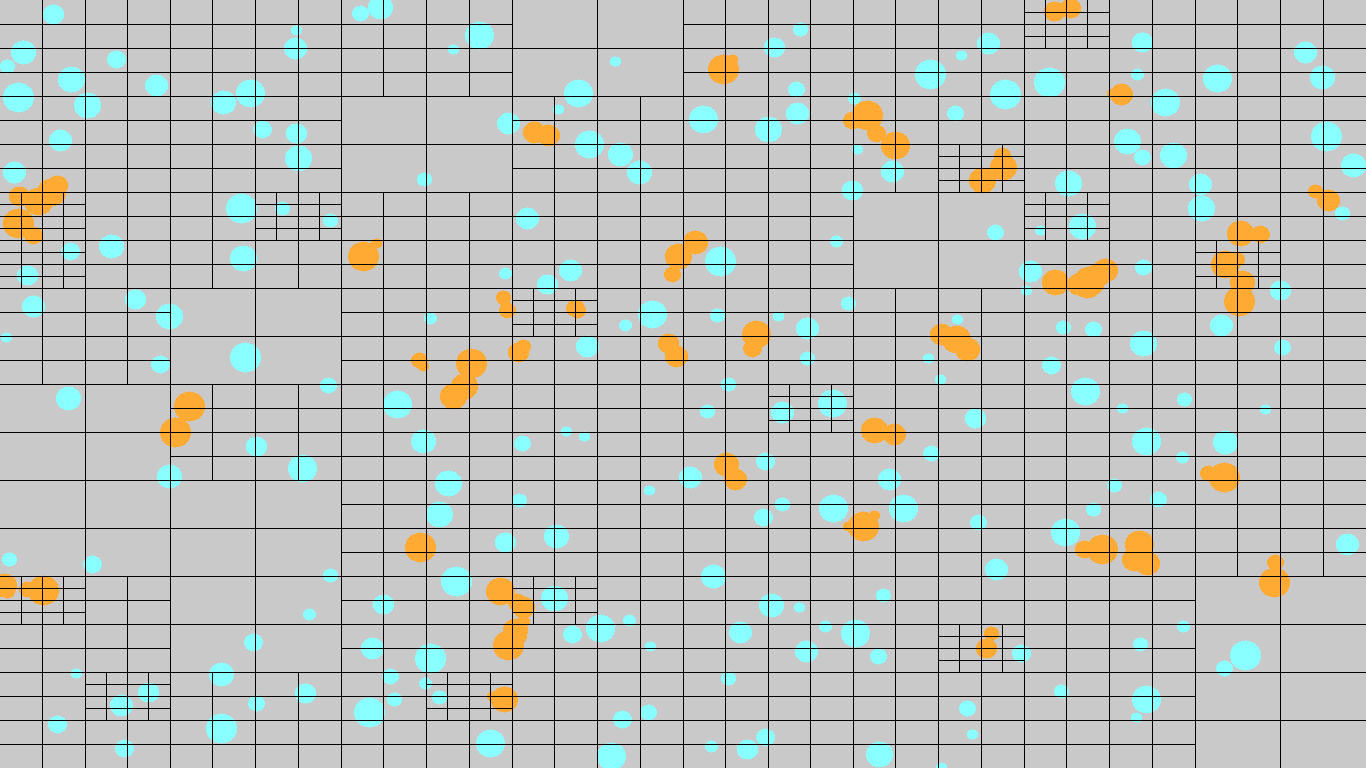
\includegraphics[width=0.8\textwidth]{./img/sim3}
	\caption{Simulation running with quadtree collision
	detection. The quadtree's boundaries are being drawn to
	demonstrate the depth of the quadtree's ``splits''.}
	\label{figure:simquad}
      \end{figure}

    \section{Algorithms \& Complexity}
      \subsection{Collision Primitive}
	In order to detect if two particles are colliding, we require
	some primitive function to use in all collision detection
	contexts. In our case, we wrote the function
	\texttt{colliding()}. Informally, we compute the distance
	between the two circles, and then see if the radii of the points
	are overlapping. If so, then we have detected a collision.
	Clearly, the runtime of collision() is a constant time operation
	--- though we calculate the vector norm to compute distance, and
	computing the norm is an $O(n)$ operation, we argue that the
	function is still constant time since the size of $n$ does not
	vary in our use case (as the number of components of the input
	vectors will always be two).

      \subsection{Brute Force}
	Our brute-force collision detection algorithm loops through the
	list of particles in a World instance. We use the
	\texttt{combinations()} function in the popular Python library
	\texttt{itertools} to take all distinct combinations of
	particles $p_i$ and $p_j$. As discussed in class, the number of
	such combinations is ${n \choose 2}$, where $n$ is the number of
	particles in the simulation. For each pair, we call the
	\texttt{colliding()} function, and if this call returns True, we
	set the ``colliding’’ attributes of $p_i$ and $p_j$ to True.
	Python code for this algorithm can be found in
	Figure~\ref{figure:brute}.

	\par Brute force collision detection works well for small input
	values. We found that performance with 50 moving objects was
	satisfactory. After 100 objects are spawned, however, the
	framerate slows down noticeably. At $N = 200$, the simulation
	slows to a crawl. For real-time applications with lots of
	objects, this would make brute force collision detection
	unusable.

      \subsection{Quadtree}
	By contrast, our quadtree collision detection algorithm uses the
	world to instantiate a quadtree containing all of the particles.
	To tell if a particle $p_k$ is currently colliding with another,
	we recurse downward into the quadtree from the root node to the
	lowest containing node for $p_k$. Each of the nodes encountered
	along this path has a list of particles, and for each of these
	particles $p_j$ we call \texttt{colliding($p_k$, $p_j$)} and set
	the colliding attribute to true if it returns True.  Python code
	for this algorithm can be found in Figure~\ref{figure:quadtree}.

	\par We argue that the quadtree performs in $O(n*log(n))$ time.
	Our quadtree implementation has superior experimental
	performance in comparison to the brute force solution. As shown
	in our data, the quadtree handles $N = 200$ easily, maintaining
	a high framerate.  Though our quadtree implementation is
	considerably faster than the brute force collision detection, it
	falls short of the potential theoretical performance gains. We
	attribute this to a number of factors, not the least of which is
	how the quadtree is reconstructed on every frame, completely
	sans caching. In addition, we are copying more information than
	necessary into the tree. Lastly, the expressiveness and
	terseness of Python’s syntax comes at a cost: there is high
	computational overhead in comparison to compiled languages.


    \begin{figure}[hb]
      \begin{minted}[linenos, numbersep=5pt,
	frame=lines, framesep=2mm]{python}
def brute_check(world):
    for p in world.particles:
	p.collide = False
    for (p1, p2) in combinations(world.particles, 2):
	if colliding(p1, p2):
	    p1.collide = True
	    p2.collide = True
      \end{minted}
      \caption{The brute force collision detector algorithm.}
      \label{figure:brute}
    \end{figure}

    \begin{figure}
      \begin{minted}[linenos, numbersep=5pt,
	frame=lines, framesep=2mm]{python}
def quadtree_check(world):
    for p in world.particles:
	p.collide = False

    qt = Quadtree(world)

    for p in world.particles:
	current = qt.root
	while True:
	    if current.hasColliding(p):
		p.collide = True
	    if current.children is not None:
		current = current.children[current.quadrant(p)]
	    else:
		break
      \end{minted}
      \caption{The quadtree collision detector algorithm.}
      \label{figure:quadtree}
    \end{figure}

    \section{Implementation}
      \subsection{Pygame}
	All rendering was handled by the \texttt{pygame} library.
	\texttt{pygame} abstracts away (some) of the complications of
	rendering graphics. In particular, it saved us the trouble of
	working with the Python OpenGL interface, which caused us many
	difficulties during the early stages of our project.

      \subsection{Model-View-Controller}
	We separated the implementation of our demo into several
	different components using the MVC design pattern. Code that
	handles rendering the simulation is in \texttt{front.py}, logic
	related to the current state of the simulation is in
	\texttt{model.py}, and code that facilitates communication
	between the frontend and the backend is stored in
	\texttt{controller.py}. In addition to making the code better
	organized, this also made it easier for us to collaborate, as
	the modular nature of this design pattern allowed us to split
	our development up into the three facets of the program.

      \subsection{cProfile}
	All profiling is facilitated by the cProfile library, which is
	packaged with Python out of the box. cProfile offers information
	on the number of executions of Python functions and the cumulative
	time spent executing those functions. We found this library very
	amenable to the task of analyzing the performance of our
	simulation in a fine-grained way. The timing technique used in
	this class's labs was ``integration''-style timing, while
	cProfile, as a proper profiling tool, offers ``unit''-style
	timing.

      \subsection{Git Branches}
	We also acquainted ourselves with the use of branches for
	collaborative development for this project. For instance, one of
	us would edit the MVC's model on the ``model'' branch, while the
	other would make necessary changes to the view on the ``gui''
	branch. Combining the resultant code was a matter of merging our
	branches together, rather that performing automerges due to
	conflicting commits on our separate development machines. In our
	view, this followed one of the core tenets of Git: ``Branch
	early, branch often.''

    \section{Results}
      In Figure~\ref{figure:graphs}, we can see the difference in
      scaling between the brute-force method and the quadtree method.
      The former scales rapidly, and by 500 particles results in a poor
      framerate. However, the scaling of the quadtree-based collision
      detection method is far more gentle, and though the latency of the
      \texttt{check()} call is still visible in the framerate for 500
      particles, it is far faster than that of the brute-force method.

      \begin{figure}
	\centering
	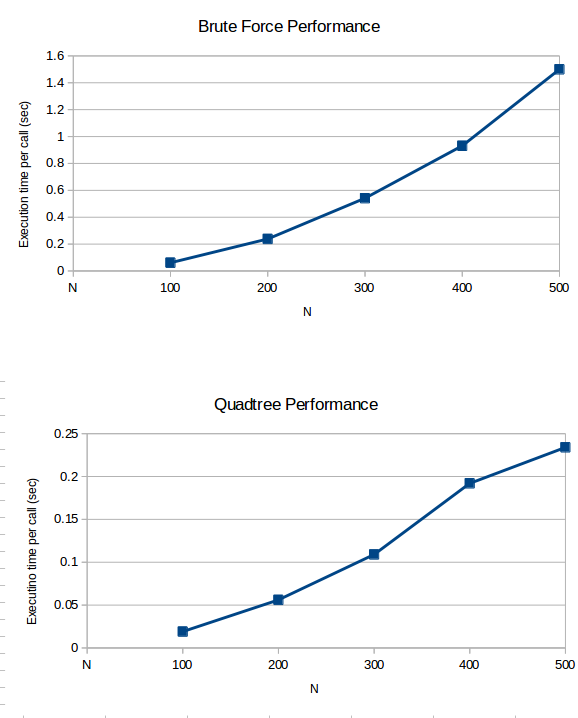
\includegraphics[width=0.8\textwidth]{./img/graphs}
	\caption{Graphs of brute-force and quadtree collision detection
	performance over number of particles in simulation. The y-axis
	represents the average execution time of the call to the
	\texttt{check()} method (taken from cProfile).}
	\label{figure:graphs}
      \end{figure}

    \newpage
    \section{Conclusion}
	We had a number of challenges and takeaways from completing this
	project:
	\begin{itemize}
	  \item Originally, we intended to write a 3D simulation using
	    an Octtree (the 3D analogue of a quadtree). However, we
	    faced difficulties using the Python OpenGL bindings,
	    especially given the multitude of development platforms we
	    were using for construction of the simulation. As a result
	    of these difficulties, we chose to reduce the scope of our
	    project to 2D and use a more ``Pythonic'' library for
	    rendering. This proved to be a wise choice: without the
	    constant hassle of 3D rendering, we were able to focus on
	    the details of algorithm implementation and analysis.
	  \item In spite of our admittedly inefficient
	    quadtree implementation, performance was still vastly
	    superior to brute force detection.  Even reconstructing,
	    redrawing, and traversing a quad-tree is way better than the
	    naive approach. This shows that, in this case, a clever
	    algorithm trumps a highly optimized implementation. There is
	    simply no substitute for a less-complex algorithm.
	  \item One lesson we learned is how much one poor design
	    decision can cascade into even more problems. This is
	    exemplified by our choice to have our choice of collision
	    detection algorithm chosen in \texttt{controller.py}, which
	    ended up making it very difficult for the frontend to
	    ``talk’’ with the quadtree. Since we needed access to the
	    state of the quadtree in order to draw it, we should have
	    instead opted to instantiate it inside of the world. We
	    ended up doing a number of ugly kludges to get around this,
	    including modifying frame drawing logic in dangerous ways.
	\end{itemize}

\end{document}




%\inputminted[fontsize=\footnotesize]{python}{../src/BST.py}
% \begin{multicols}{3}
%     \inputminted[fontsize=\footnotesize]{python}{../output/traverseoutput}
% \end{multicols}
% \csvautotabular{../data/runs.csv} \\
% \includegraphics[scale=0.40]{../output/rbtgraph.png}
% \begin{minipage}[t]{0.3\textwidth}
%     \VerbatimInput[fontsize=\scriptsize]{delete1.txt}
% \end{minipage}
% \begin{minipage}[t]{0.3\textwidth}
%     \VerbatimInput[fontsize=\scriptsize]{delete2.txt}
% \end{minipage}
